\documentclass[12pt]{article}
\usepackage{xcolor}
\usepackage{hyperref}
\hypersetup{
    colorlinks = true,
    citecolor = {black}}
\usepackage{wrapfig}
\setlength{\parindent}{0pt}
\usepackage[font = {small, it}]{caption}
\DeclareCaptionLabelFormat{cont}{#1~#2\alph{ContinuedFloat}}
\captionsetup[ContinuedFloat]{labelformat=cont}
\usepackage{tgtermes}
\usepackage{setspace}
\usepackage{gensymb}
\doublespacing
\usepackage{graphicx}
\usepackage{float}
\usepackage[utf8]{inputenc}
\usepackage[backend=biber,style=apa,autocite=inline]{biblatex}
\usepackage{fancyhdr}
\pagestyle{fancy}
\lhead{Paper 1}
\rhead{Victor M. Poulsen, Studie Nr.: 201707639}

\DeclareLanguageMapping{english}{english-apa}
\addbibresource{report.bib}

\title{Human Computer Interaction}
\author{Victor Møller Poulsen, Studie Nr.: 201707639}

\begin{document}
\maketitle
\leavevmode

\section{Abstract}
This paper presents a prototype Streamlit app which teaches a Gelman
\autocite{gelman2020bayesian} inspired Bayesian workflow
in R with the package brms \autocite{Burkner2017} and in Python with the
package pyMC3 \autocite{Salvatier2016}. The app is built with theories from user
experience (UX) in mind and relies on a well-documented and reproducible code-base. The app is
aimed at users who are already familiar with Bayesian analysis in either R
(brms) or Python (pyMC3) and should be used as an introduction to the
implementation that the user is unfamiliar with. The app has several
interactive elements, including optional sections, flexible plots and quizzes. \\
Link to Streamlit: \href{https://share.streamlit.io/victor-m-p/bayesworkflow/main/BayesWorkflow.py}{Stremlit app}\\
Link to Github: \href{https://github.com/victor-m-p/BayesWorkflow}{Github page}

\tableofcontents
\newpage
\section{Introduction}

The main idea with this app is to teach users who know how to conduct a Bayesian analysis in one coding
language how to conduct a similar analysis in the other coding language. This is something
that I had to figure out when we transitioned from using R and brms for Bayesian analyses
on the Cognitive Science bachelor's degree to using Python and pyMC3 on the Cognitive Science
master's degree. There are lots of great resources and examples both online and in books for both
brms and pyMC3 independently, but I have so far not found any resources that
directly translate between
the two. That is the niche that this Streamlit app is intended to occupy.

\vspace{5mm}

Besides differing in content from books and online resources, this app is also interactive.
This is important because interactive elements facilitate user engagement and
lead to a sense agency for the user \autocite{janlert2017meaning}. It is also important, because a healthy
Bayesian workflow is iterative and non-linear \autocite{gelman2020bayesian}.
Interactive elements allow the user to select what they want to engage
with, and they provide the option to avoid in-depth discussions in other places.
It thus saves a lot of
clutter from the app, because we can avoid displaying everything at once.
It also means that the app is flexible enough to accomodate various use cases.
This is something that we will return to later.
In sum, the hope is that the app can both support extensive functionality and retain high usability.

\vspace{5mm}

This is where Streamlit becomes relevant. Streamlit is a Python package which allow users
to launch interactive web applications to showcase analyses. It thus fulfills the same function
that Shiny fulfills in the coding language R. Streamlit is developing rapidly however,
and already appears to support more diverse options than Shiny. For instance,
the expandable sections that I use throughout the app were released in 2021. I chose to
use streamlit because it is an exciting and developing tool which suit the
needs of the intended product.

\section{Target Group}
Obtaining knowledge and understanding of the target group for a product is among the
most important steps in creating a useful product
\autocite[13]{mills1992macintosh}.
The target group for this app is people who are familiar with Bayesian statistics and know
how to conduct a Bayesian analysis in either R (brms) or Python (pyMC3). The idea is to
conduct (almost) identical analyses in the two languages, such that users can
transfer what they already know in one language to the other language.
Explanations are targeted more towards users who want to transition from R (brms)
to Python (pyMC3) than the other way. This is because I have kept Cognitive Science students
in mind as the primary audience. Most Cognitive Science students have been
taught Bayesian statistics in the R programming language, as implemented in the
brms package. I am in the privileged position of knowing my audience well. I
have both (1) been taught Bayesian statistics in R on the Cognitive Science
Bachelor's degree, and (2) taught as instructor on the Bachelor's course in which
the students learn Bayesian statistics in R.
While the app is mainly designed with Cognitive Science students in mind,
the app should also be useful for users outside of Cognitive Science.
Python and R are the two largest Data Science programming
languages, and as such it is common for Data Scientists to code in both
languages.

\section{Intended Usage}
The first reasonable use case (\emph{UC1}) is to use the app as a one-time
thorough introduction, where users should ideally run their own code in Python and/or R
while following the analysis on the app. This should be relatively easy since I provide reproducible code
for all parts of the analysis, which can be easily copied to clipboard from the expandable
code-chunks. Users do not need to manually select the code they want to copy but can simply click
the text selection icon in the upper-right corner of the code-chunks. This also
preserves code-formatting, such that indentation is preserved when users paste
code into their local instance of either R or Python.
For \emph{UC1} the user will have to interact with the app,
and will utilize the full functionality.

\vspace{5mm}

The second plausible use case (\emph{UC2}) is to use the app repeatedly as a reference
while the user is conducting their own analysis in either pyMC3 or brms. The user can quickly glance through the
app to be reminded of how a good Bayesian workflow can look for either implementation.
I have also included a section with references that I have found helpful for both pyMC3 and brms,
and as such the user can also use the app as a gateway to more advanced analyses.
For this use case the user might not want to expand the optional sections,
but simply glance through the plots and headers to quickly find what they are looking for.
For this use case, only a small part of the functionality in the app is used.

\section{Design Philosophy}
The design philosophy for the app is naturally related to the content that it attempts to convey and
introduce to the user. It is also designed to facilitate both \emph{UC1} and
\emph{UC2}. The design philosophy burrows from the Pragmatic/Hedonic model of
User Experience (UX) which is described in \textcite{hassenzahl2010experience} as well as the design
principles outlined in \textcite{mills1992macintosh}.

\vspace{5mm}

Firstly, the app is designed with a philosophy of \emph{avoiding clutter} in mind.
The importance of this is emphasized throughout \textcite{mills1992macintosh}.
I have hidden everything that I think is not necessary for navigating the app
in expandable sections. I wanted to avoid cluttering the
app with text specifically since this can feel intimidating and could scare users away.
If users want to use the app in line with \emph{UC1} they will have to interact with the optional
elements and decide to see the code-chunks and the optional explanatory sections.
If these were shown by default, \emph{UC2} would not be facilitated well by the app.

\vspace{5mm}

Secondly, the app is designed with \emph{consistency} in mind.
The importance of consistency is discussed in
\textcite[7]{mills1992macintosh}
where they highlight that consistency allows users to transfer knowledge from one
application to another. In our case, since we only have one app, what will be important is
that users can transfer what they have learned in one section to other sections.
In other words, I am aiming for the app to be consistent within itself
\autocite[8]{mills1992macintosh}.

\vspace{5mm}

The users will quickly learn that there are three types of expandable boxes in the app:
“Code-Monkey”, “Language-Learner” and “Concept-Guru”. Each of these expandable sections
allow the user to access different types of additional info. When clicked, the “Code-Monkey”
sections will pop out and show reproducible code, “Language-Learner” sections go into more detail
about how R (brms) differ from Python (pyMC3) while “Concept-Guru” sections discuss Bayesian analysis
more generally. Python and R placement on the page is consistent in the sense
that everything which relates to R (e.g. plots and code) is located in the
right column, while everything related to Python is located in the left column
(see \emph{Fig. 1} and \emph{Fig. 2} below).
The order of presentation is also consistent throughout.
Each subsection starts with a header and is then followed by a brief text.
Below this are plots or outputs from Python and R, and only after this will the user find
the optional sections. These are also presented in consistent order, such that “Code-Monkey” comes first,
“Language-Learner” second and “Concept-Guru” comes last. For examples of this
consistent format, see \emph{Fig. 1} and \emph{Fig. 2} below.
Lastly, each expandable section
has a unique icon associated with it. This has been implemented to make it easier for the
user to navigate the page (see \emph{Fig. 1 \& Fig. 2}). \textcite[223-255]{mills1992macintosh} focus
heavily on the importance of icons. One highlighted advantage of icons is that users typically
will recognize images and icons faster than they will read text
\autocite[244]{mills1992macintosh}.

% consistency image
\begin{figure}[H]
    \centerline{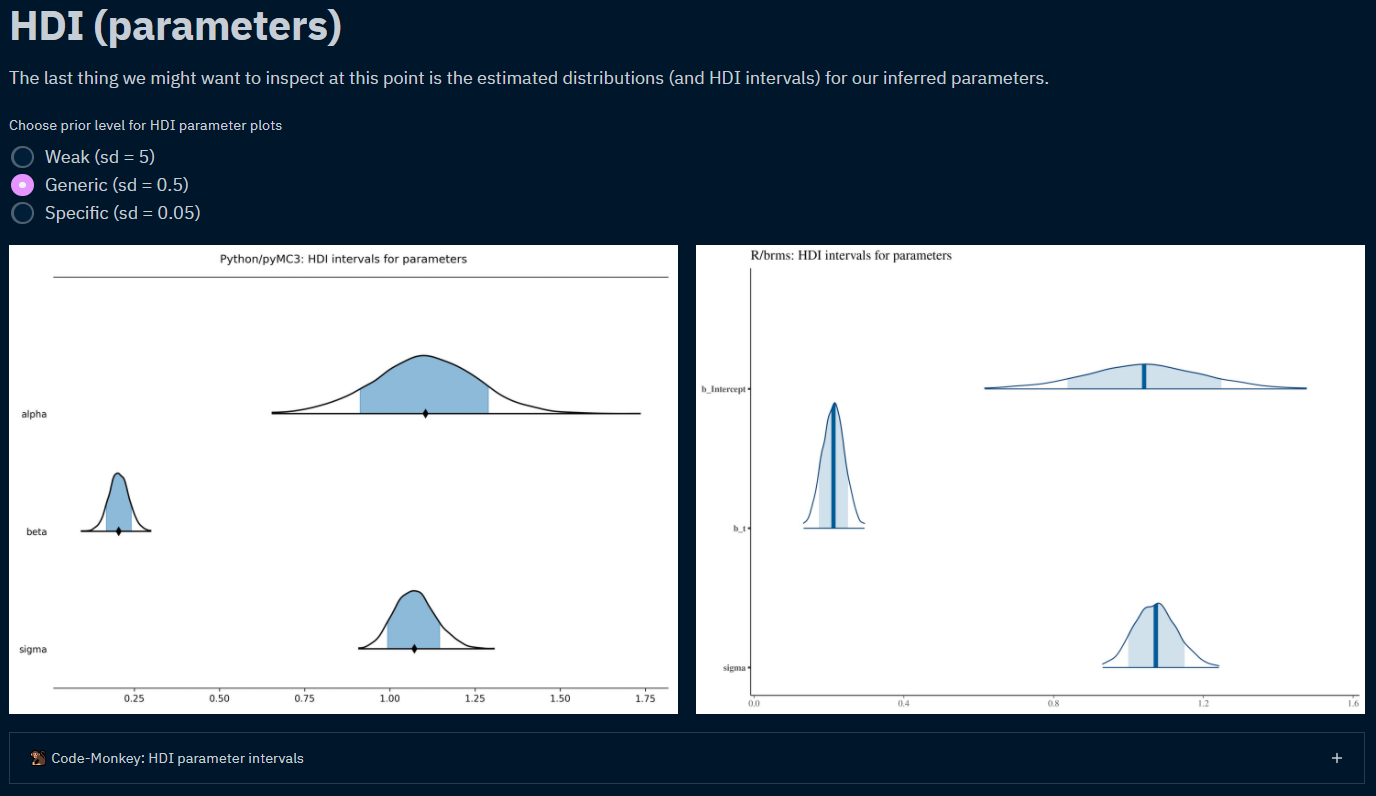
\includegraphics[scale = 0.5]{../img/Pretty-Consistent.png}}
    \caption{Screen capture from
	    \href{https://share.streamlit.io/victor-m-p/bayesworkflow/main/BayesWorkflow.py}{Streamlit}.
    Shows the consistent, pretty and simple layout on the app.
    Each subsection starts with a header and a brief text.
    Then the user makes a selection (the \emph{Generic} prior is chosen by
    default). A plot or figure is then shown based on the selection (left: Python, right:
    R). At the bottom, we see an expandable "Code-Monkey" section with a monkey icon.
    }
\end{figure}


\vspace{5mm}

Third, the app should be \emph{pretty} and \emph{simple}. These are general
and obvious design principles which are discussed in
\textcite{tractinsky2000beautiful} as well as
\textcite[25-26]{hassenzahl2010experience}.
I have created a custom color-theme for the app, which I think makes the app more interesting
than with the standard white theme. I have also tried to make the formatting both inside
Streamlit, and for the R and Python plots pretty and consistent (see \emph{Fig.
1} above \& \emph{Fig. 2} below). Considerations around making
the app engaging
and pretty is another reason why I show plots by default and hide most text and code by default.
Plots and figures are just more interesting and attention-grabbing than
written text and code.
I hope that users will find that the app and the content on it is pretty,
something that is understood to be an important driver
in creating an enjoyable experience \autocite[65]{hassenzahl2010experience}.

\section{Interaction}
There are three basic types of interaction implemented in the app
at this point. They provide a relatively high level of
interactability, with adaptable outputs that are contingent on
user selection \autocite{janlert2017meaning}.

\vspace{5mm}

Firstly, the user can choose which model and prior to see analysis for.
Plots and figures from R and Python are shown by default and cannot be toggled off by the user.
However, the user can influence what is shown in plots. In most cases the user can choose
among different prior options that have been used to fit the models in the app
(see \emph{Fig. 1} above).
In some cases, the user can choose to plot the outputs of analysis between different models,
e.g. with different random effects structure and likelihood functions.
When the user makes a selection the plots and figures will change,
and the code in the “Code-Monkey” sections will also change in the cases where
the analysis code differ.
As such, the display is contingent on the actions of the user,
and there is an element of adaptability imbedded in the
app \autocite{janlert2017meaning}.


\vspace{5mm}

Secondly, the user can choose to expand the optional sections:
“Code-Monkey”, “Language-Learner” and “Concept-Guru” (see \emph{Fig. 2} below).
As we have already discussed, the “Code-Monkey” section will render code which matches the selection.
Most often, the content in “Language-Learner” and “Concept-Guru” will not
change
based on the selection of the user, because these sections contain more general considerations.

\vspace{5mm}

The degree to which a
product engages the user in interaction has been called \emph{interactiveness}
\autocite{janlert2017meaning}. Interactiveness is implemented with quizzes that the app
poses to users and the feedback that the app provides based on user answers.
These quizzes are not shown on the page by default but hide inside the
expandable boxes (see \emph{Fig. 2} below). The quiz functionality is targeted
towards \emph{UC1} where users are expected to engage with the full material on
the app. Quizzes are hidden in optional sections in order to make sure that the app can
be quickly glanced through, supporting \emph{UC2}.

\vspace{5mm}

Streamlit is often used for Data Science applications which run extremely
fast machine learning analyses or frequentist statistics. These apps are typically
interactive in the sense that when the user makes a choice, corresponding code
is executed,
which generates an output that the user sees. This means that the possibility space is almost
infinite, and as such these apps are high on interactiveness
\autocite{janlert2017meaning}. This is not the case in the prototype app that
I am presenting. In our case, no analysis code is executed live because full
Bayesian sampling is prohibitively slow. Thus, an extensive code base has been
developed from which plots and outputs are generated for several parallel analyses
(e.g. for different priors and different models). The user is shown
pre-generated outputs based on
selection. As such, the functionality, or interactability is limited to what is
already pre-run. This is a classic trade-off between functionality on one
hand (flexible options) and usability on the other (no delay in runtime).
However, \textcite{janlert2017meaning} point out that higher interactability
does not necessarily mean that a product gives the user a stronger feeling of
agency. Even though this
app only offers limited interactability in the sense discussed,
I hope that it does provide users with a
sense of agency.

\section{Code Base}
Although I have focused extensively on the user experience (UX) on the app,
the most demanding work has been to develop good example analyses and to manage an extensive
code base, which must be reproducible. I will not go too deep into that here,
as you can check the
\href{https://github.com/victor-m-p/BayesWorkflow}{Github}.
There are bash-scripts for both R and Python
which execute all the necessary scripts to run the whole pipeline
and reproduce all analysis and outputs shown on the Streamlit app. This means that if users have
the necessary packages in their local environment, they can run all R and Python analysis
with two lines of code from their terminal. This is of course unnecessary for most users,
who will just stay in the app, but it is an option for users who want to dive deeper
into the analysis and the convenience functions that I have created. It is
important not exclusively to focus on the "average" user
\autocite[14]{mills1992macintosh}.
Besides this, a well-structured code base has been absolutely necessary
in order to manage the project and ensure that all formatting is consistent.

\section{Improvements \& Testing}
An obvious improvement to the usability of the app would be to implement a consistent
color-code for the expandable sections. This would make sense
because the app uses the same three types of boxes (“Code-Monkey”, “Language-Learner” and “Concept-Guru”)
throughout. A color scheme, where each type of section has its own color-code
should make the page more intuitive to navigate. Unfortunately, this functionality
is not natively supported in Streamlit. Streamlit can be configured with CSS code,
so in principle it should be possible to implement. Unfortunately, I am unfamiliar
with CSS so there is currently no color-coding for the expandable sections.
As mentioned previously, each type of section has an associated icon,
which aims to achieve the same goal of directing the users attention.
I do think that colored sections would be more effective at this than small icons,
and would make interaction with the app easier and faster for the user.

\vspace{5mm}

With regards to feedback and interactivity there is one thing that would be ideal
to implement for the use cases that the app attempts to facilitate. At present,
the user is only quizzed with multiple choice questions (see \emph{Fig. 2}
below). This is because it is easy
to handle, since we can specify the feedback for a limited number of options.
This is what is currently supported, and it can be characterized as a
"responding" interaction type \autocite[81]{rogers2011interaction}.
Because the app attempts to teach the user code practices it would make sense to
have a system which corresponds to what is used on platforms such as DataCamp.
On DataCamp users type in code, which is then executed, and the user receives feedback
based on what the code evaluates to. This would be closer to a "conversing"
interaction type \autocite[81]{rogers2011interaction},
and would be more sophisticated than what is currently in
place. The tricky part is that the input code from the user has to be
compiled,
and not just treated as a raw string of text. Treating the input as a string
of text is infeasible because code which accomplishes the same thing can be
expressed in infinitely many ways.
There also has to be a slick interface where the user can type in the code that
they want to execute. I think that both would be difficult to implement, especially the
first one. Another reason to not support this functionality is that I would ideally
like users to code along from their own instance of R and/or Python.

% limited interaction.
\begin{figure}[H]
    \centerline{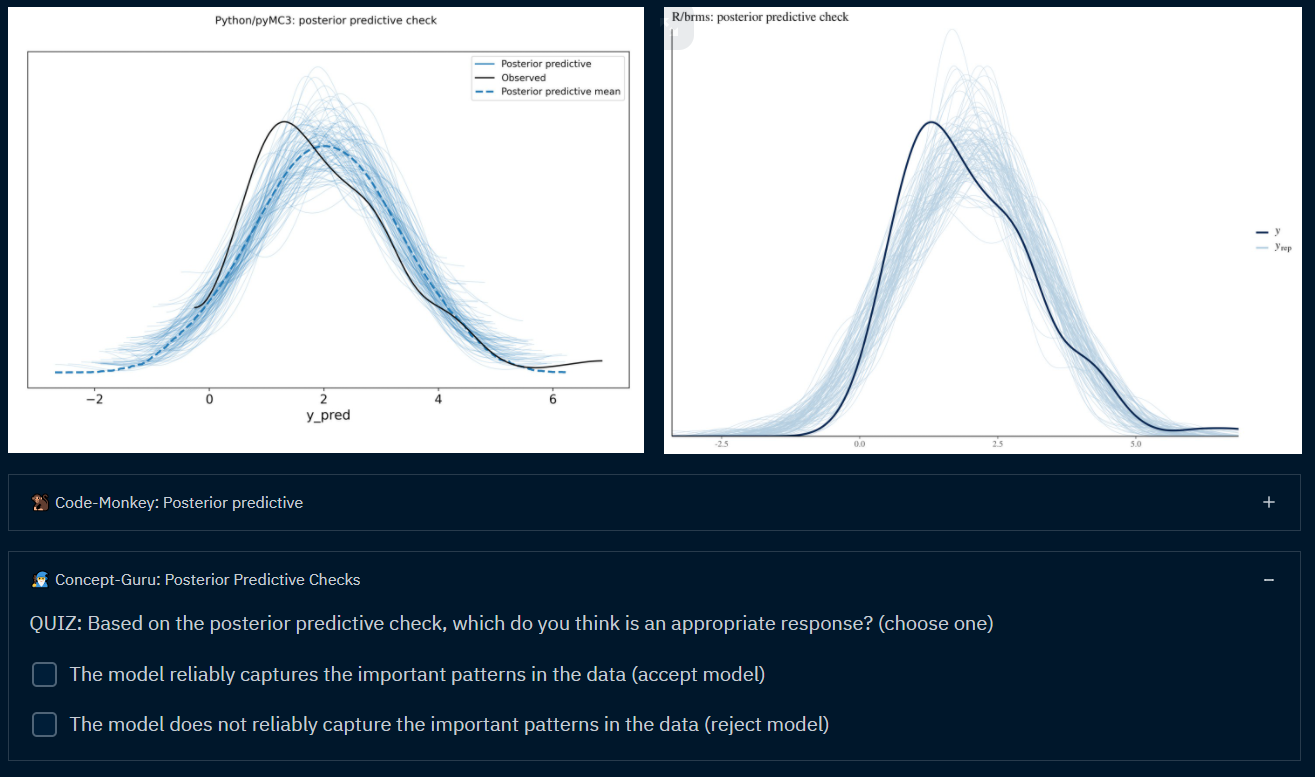
\includegraphics[scale = 0.5]{../img/Quiz-image.png}}
    \caption{Screen capture from
    \href{https://share.streamlit.io/victor-m-p/bayesworkflow/main/BayesWorkflow.py}{Streamlit}.
    Shows plots for posterior predictive checks in the top (left: Python,
    right: R). Below is an expandable "Code-Monkey" section (not expanded
    in this screen capture). At the bottom is
    an expanded "Concept-Guru" section, which has a quiz inside it.
    As can be seen, the quiz is verbal, and only supports multiple-choice answers.
    It will provide feedback once a selection has been made.
    }
\end{figure}

\vspace{5mm}

I intend to share the app in cognitive science forums once I have double checked
that everything is reproducible, well documented and otherwise complete. Hopefully,
the app will be useful to some of the students, and perhaps some outsiders will even
find their way to the app. Additionally, sharing the app should give me the chance
to receive feedback on whether the app is usable. Both whether the content is
appropriate for the target group,
and whether the format is intuitive. I intend to gather verbal feedback,
although I know that this is not the ideal testing condition.
It is however a realistic approach to obtaining some useful feedback.

\vspace{5mm}

There are at least two ways of gathering feedback that would be more thorough
than simply obtaining verbal feedback. Firstly, one could attempt a quantitative evaluation,
e.g. based on A-B testing, eye-tracking data and statistical analysis.
A good example of this approach can be found in \textcite{sutcliffe2016}.
A better approach in this initial stage might be to simply observe users who interact
with the app. \textcite{norman1999} has argued that the best way of finding
out how users engage with products is to simply observe them engage with products.
I think this is true in our case, where the main question of interest at this
point is how users engage with the app (qualitatively), rather than a
quantitative measure, such as time spent on the app.

\section{Conclusion}
This paper has introduced a Streamlit app which teaches a Bayesian workflow in R (brms)
and Python (pyMC3). The app is designed for users who are already familiar with Bayesian
analysis in either R (brms) or Python (pyMC3). The app focuses on building a bridge
between the implementations in the different languages and packages.
The app supports limited interaction through selection boxes, and expandable
sections for the user who wants to dive deeper. The app also attempts to engage
the user with quizzes and provides feedback based on answers. The app is designed with
a philosophy of consistency, simplicity and beauty in mind. Users who want to
go further than the app supports can consult a well-organized code-base at
\href{https://github.com/victor-m-p/BayesWorkflow}{Github}.
\printbibliography
\end{document}


